\chapter{Friction-strain profiles}\label{sec:data_stretch_profiles}
Friction-strain profiles for the dataset for the Honeycomb
(\cref{fig:fric_strain_hon}), Tetrahedron (\cref{fig:fric_strain_pop}) and
Random walk (\cref{fig:fric_strain_RW}) patterns respectively. The friction-strain
profiles are computed as a mean over the three normal loads used in the dataset and plotted against
the strain relative to the rupture strain. The legends show the names for each
pattern and the corresponding (absolute) rupture strain. The data has been
interpolated with a cubic spline interpolation in order to visualize the
approximate shape of the continuous curve.


% Honeycomb
\begin{figure}[H]
    \centering
    \begin{subfigure}[b]{0.49\textwidth}
        \centering
        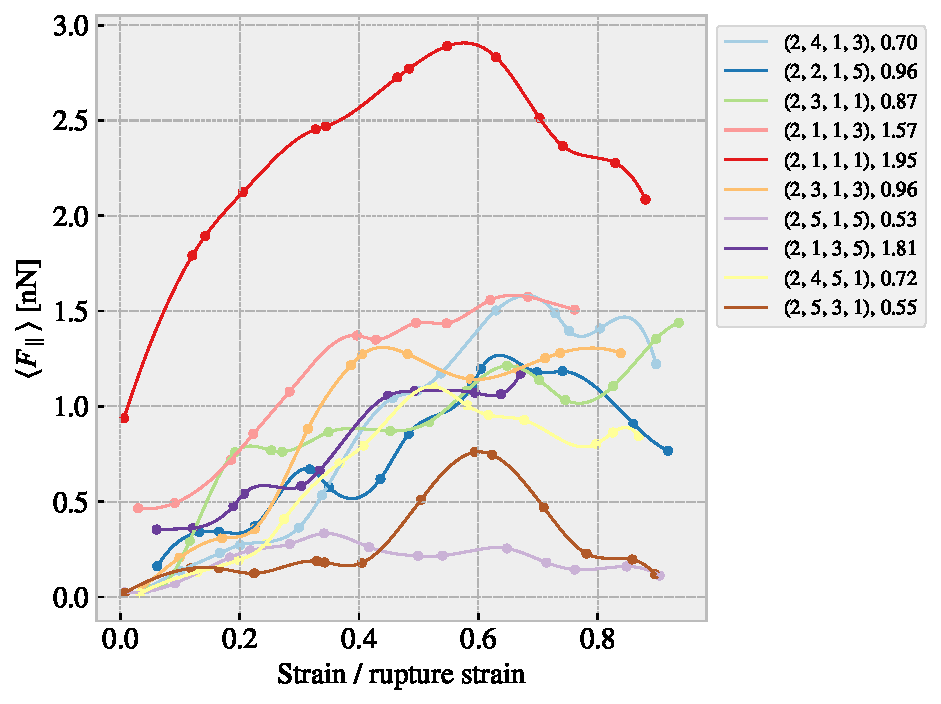
\includegraphics[width=\textwidth]{figures/stretch_profiles/honeycomb/SP_0_honeycomb.pdf}
        \caption{}
        % \label{fig:}
    \end{subfigure}
    \hfill
    \begin{subfigure}[b]{0.49\textwidth}
        \centering
        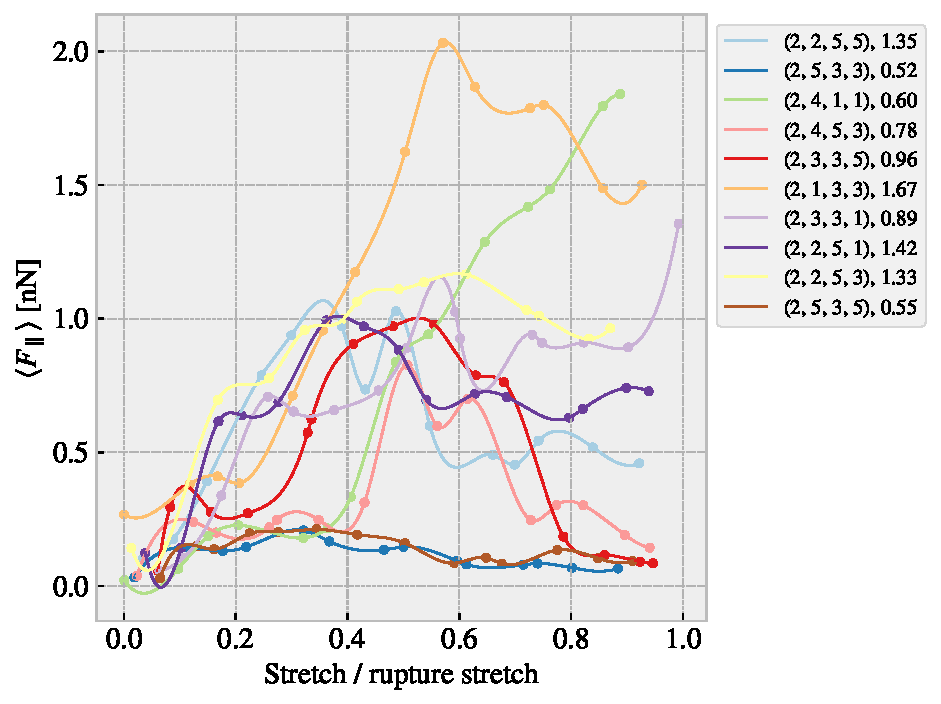
\includegraphics[width=\textwidth]{figures/stretch_profiles/honeycomb/SP_1_honeycomb.pdf}
        \caption{}
        % \label{fig:}
    \end{subfigure}
    \hfill
    \begin{subfigure}[b]{0.49\textwidth}
        \centering
        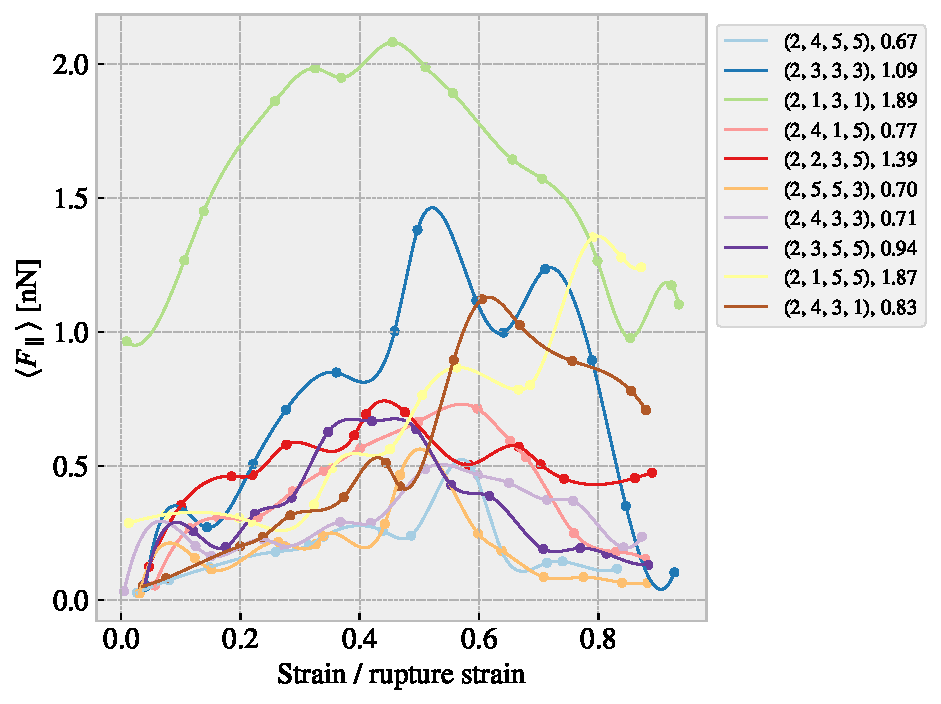
\includegraphics[width=\textwidth]{figures/stretch_profiles/honeycomb/SP_2_honeycomb.pdf}
        \caption{}
        % \label{fig:}
    \end{subfigure}
    \hfill
    \begin{subfigure}[b]{0.49\textwidth}
        \centering
        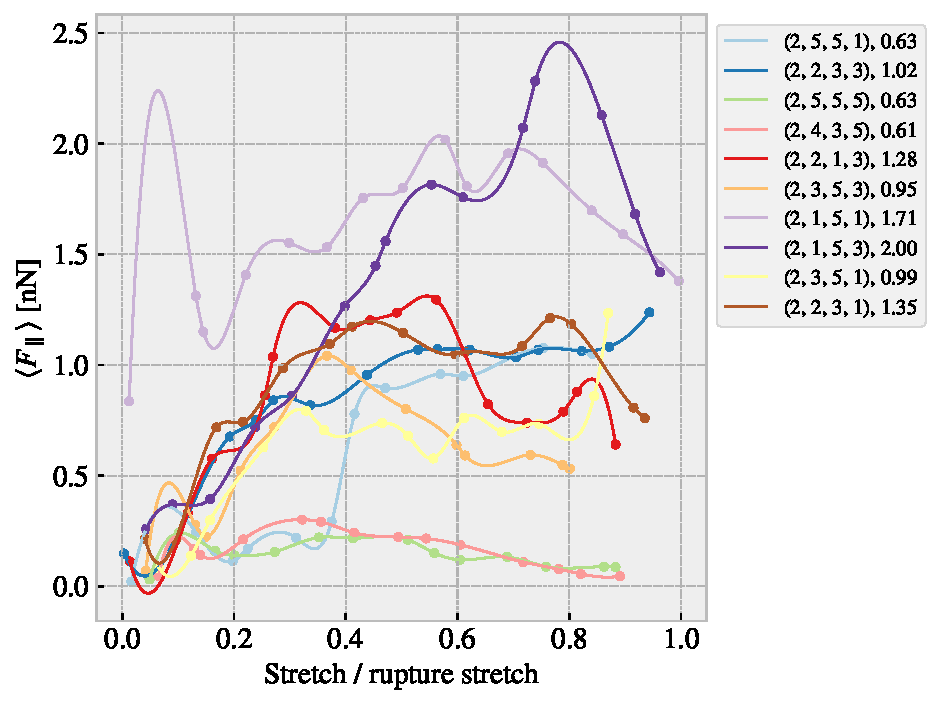
\includegraphics[width=\textwidth]{figures/stretch_profiles/honeycomb/SP_3_honeycomb.pdf}
        \caption{}
        % \label{fig:}
    \end{subfigure}
    \hfill
    \caption{Honeycomb friction-strain profiles.}\label{fig:fric_strain_hon}
\end{figure}


%Popup
\begin{figure}[H]
    \centering
    \begin{subfigure}[b]{0.49\textwidth}
        \centering
        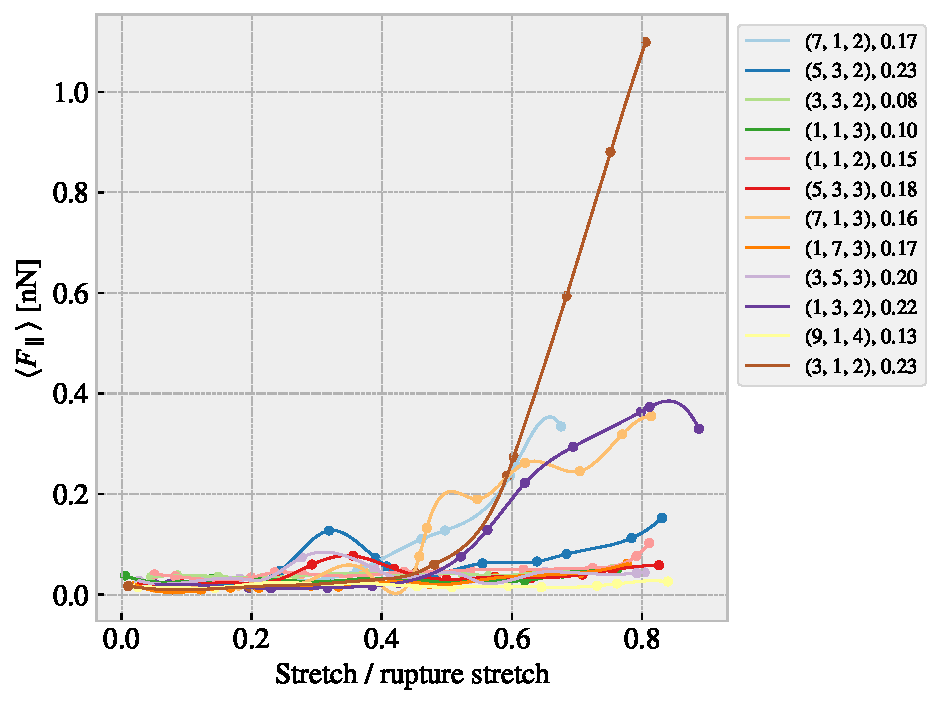
\includegraphics[width=\textwidth]{figures/stretch_profiles/popup/SP_0_popup.pdf}
        \caption{}
        % \label{fig:}
    \end{subfigure}
    \hfill
    \begin{subfigure}[b]{0.49\textwidth}
        \centering
        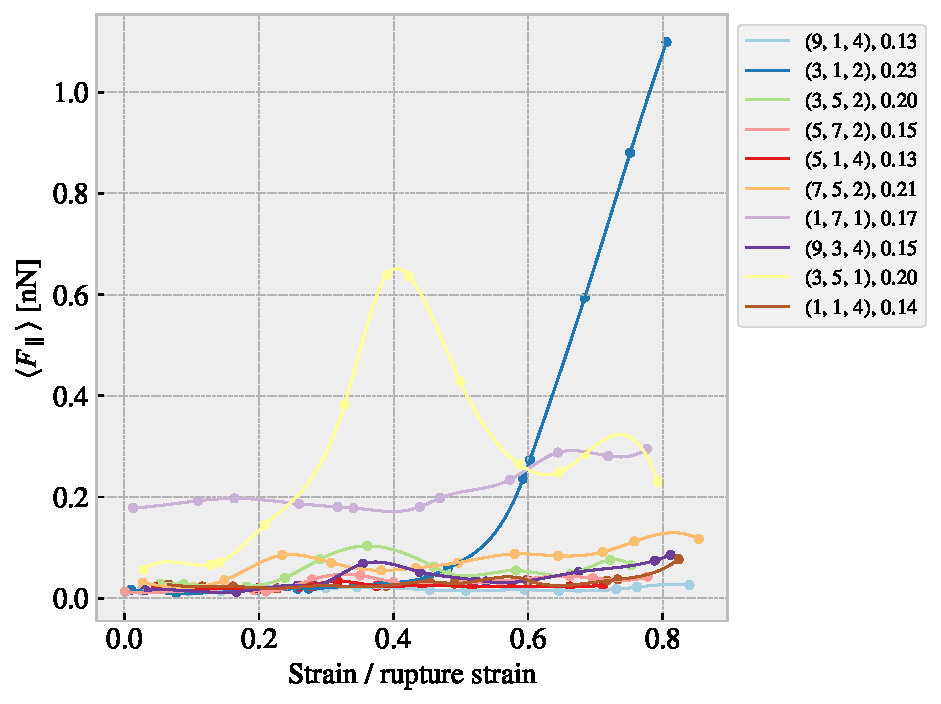
\includegraphics[width=\textwidth]{figures/stretch_profiles/popup/SP_1_popup.pdf}
        \caption{}
        % \label{fig:}
    \end{subfigure}
    \hfill
    \begin{subfigure}[b]{0.49\textwidth}
        \centering
        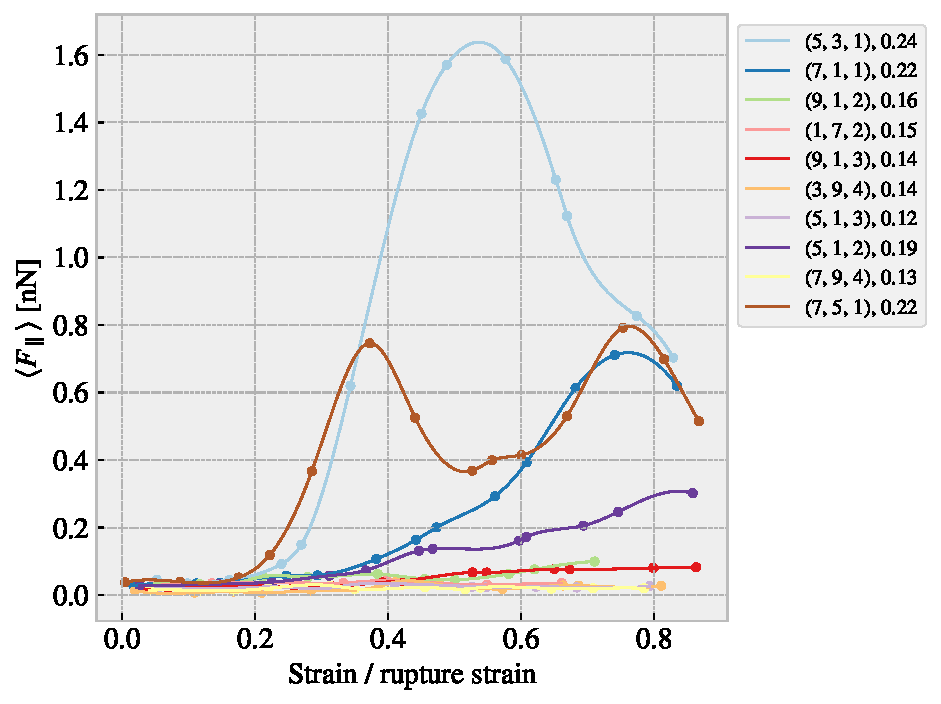
\includegraphics[width=\textwidth]{figures/stretch_profiles/popup/SP_2_popup.pdf}
        \caption{}
        % \label{fig:}
    \end{subfigure}
    \hfill
    \begin{subfigure}[b]{0.49\textwidth}
        \centering
        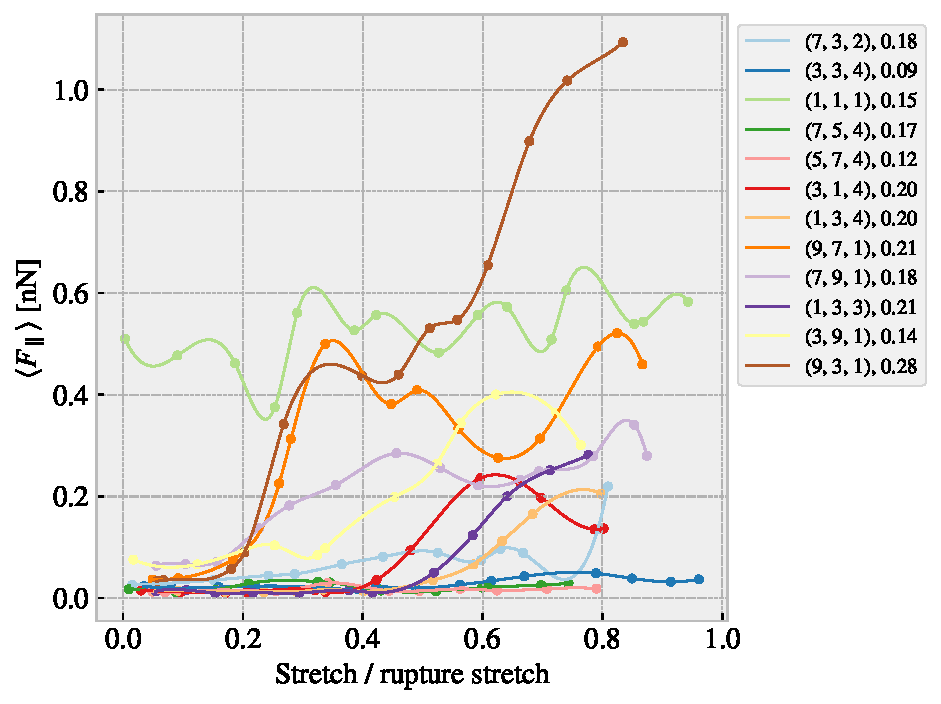
\includegraphics[width=\textwidth]{figures/stretch_profiles/popup/SP_3_popup.pdf}
        \caption{}
        % \label{fig:}
    \end{subfigure}
    \hfill
    \begin{subfigure}[b]{0.49\textwidth}
        \centering
        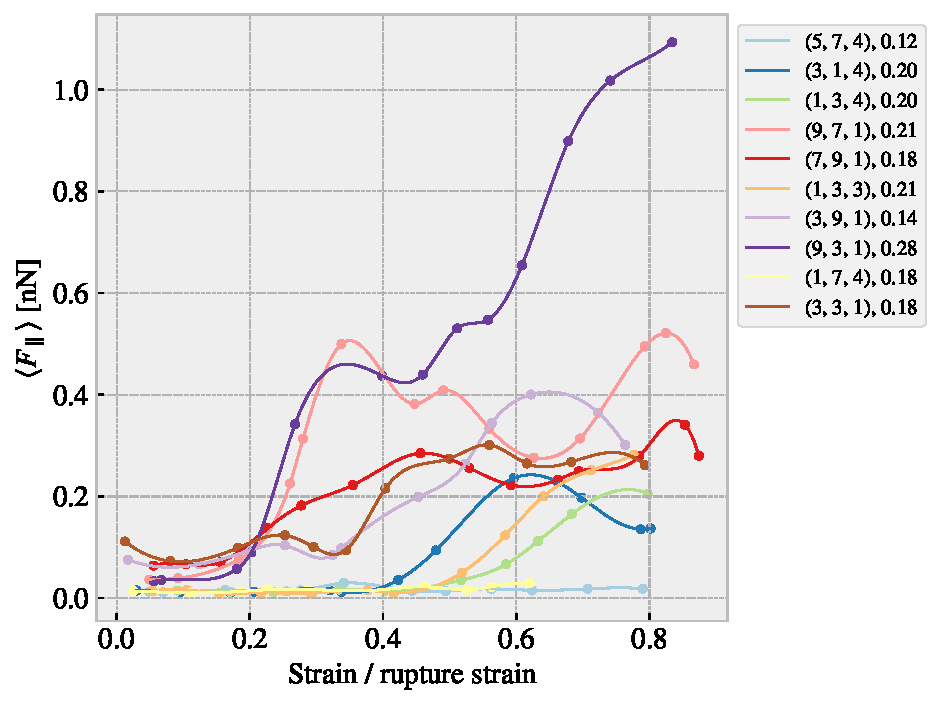
\includegraphics[width=\textwidth]{figures/stretch_profiles/popup/SP_4_popup.pdf}
        \caption{}
        % \label{fig:}
    \end{subfigure}
    \hfill
    \begin{subfigure}[b]{0.49\textwidth}
        \centering
        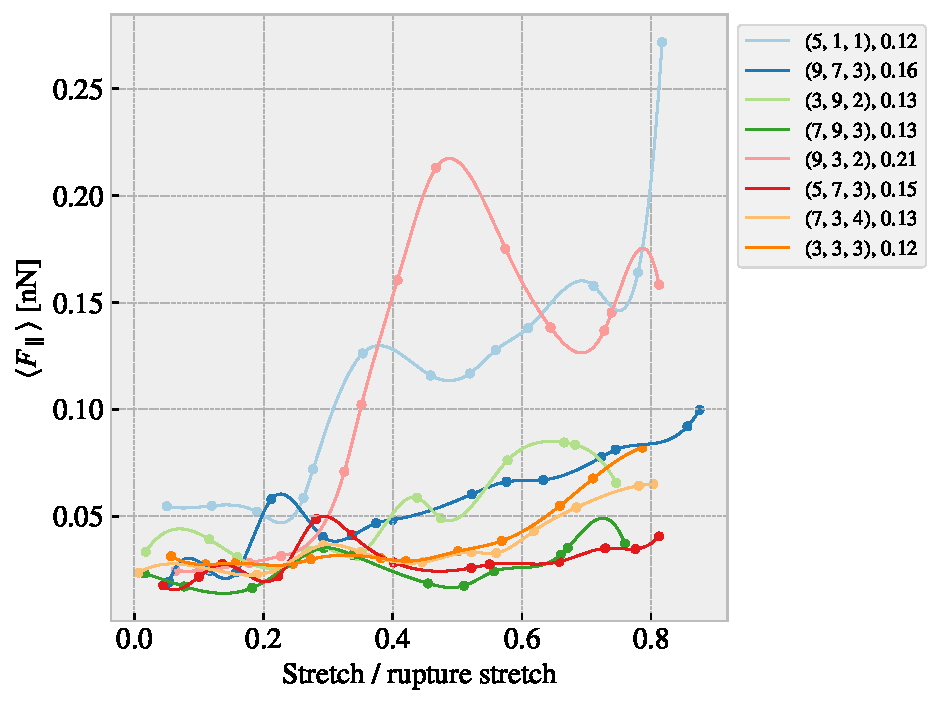
\includegraphics[width=\textwidth]{figures/stretch_profiles/popup/SP_5_popup.pdf}
        \caption{}
        % \label{fig:}
    \end{subfigure}
    \hfill
    \caption{Tetrahedron friction-strain profiles.}\label{fig:fric_strain_pop}
\end{figure}



%RW
\begin{figure}[H]
    \centering
    \begin{subfigure}[b]{0.49\textwidth}
        \centering
        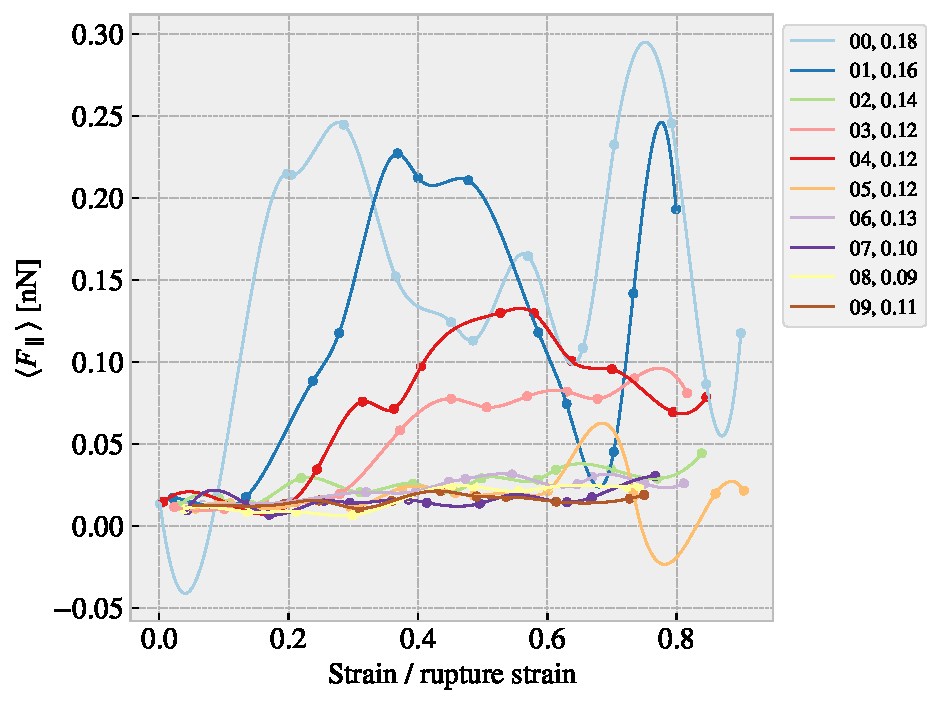
\includegraphics[width=\textwidth]{figures/stretch_profiles/RW/SP_0_RW.pdf}
        \caption{}
        % \label{fig:}
    \end{subfigure}
    \hfill
    \begin{subfigure}[b]{0.49\textwidth}
        \centering
        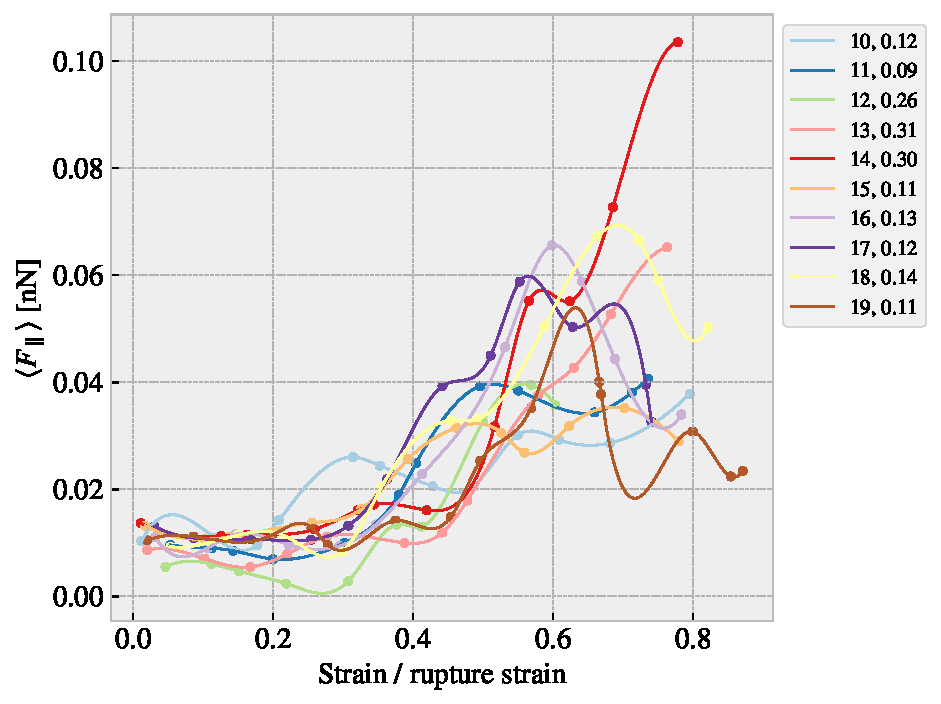
\includegraphics[width=\textwidth]{figures/stretch_profiles/RW/SP_1_RW.pdf}
        \caption{}
        % \label{fig:}
    \end{subfigure}
    \hfill
    \begin{subfigure}[b]{0.49\textwidth}
        \centering
        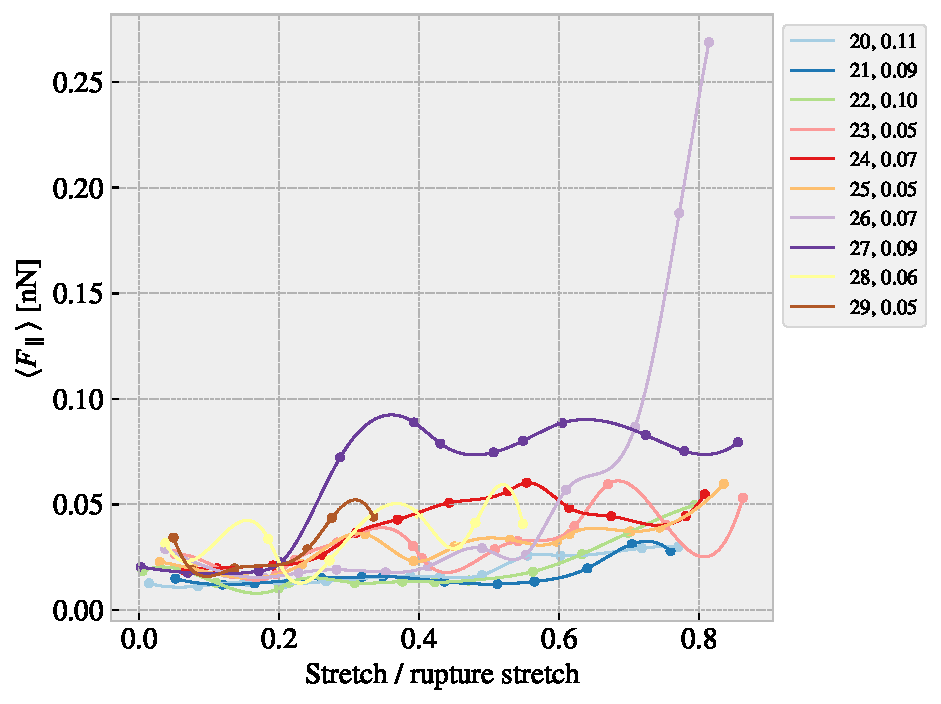
\includegraphics[width=\textwidth]{figures/stretch_profiles/RW/SP_2_RW.pdf}
        \caption{}
        % \label{fig:}
    \end{subfigure}
    \hfill
    \begin{subfigure}[b]{0.49\textwidth}
        \centering
        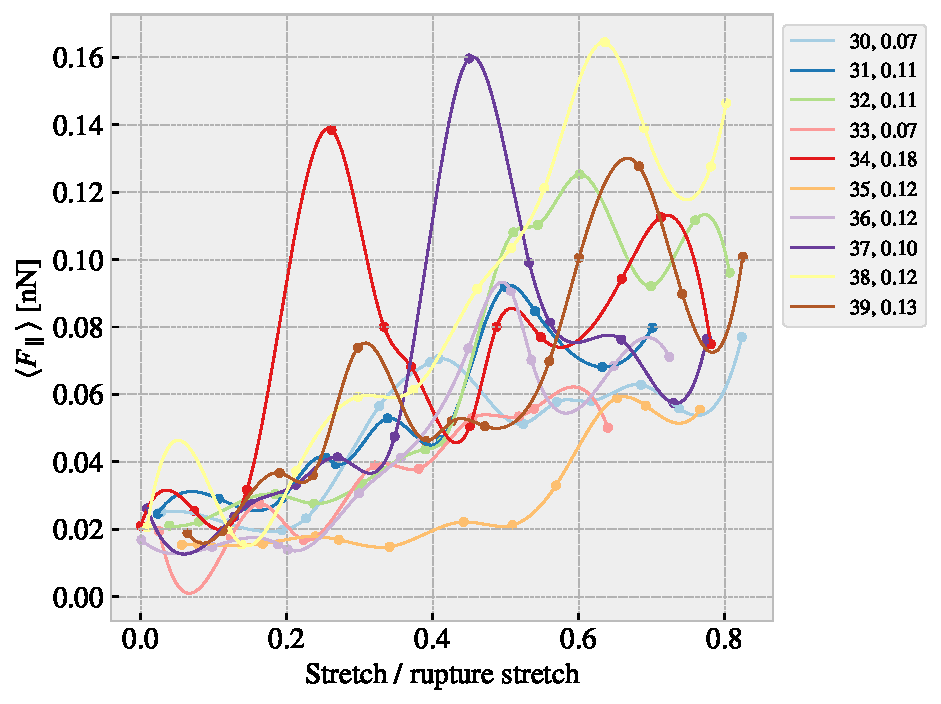
\includegraphics[width=\textwidth]{figures/stretch_profiles/RW/SP_3_RW.pdf}
        \caption{}
        % \label{fig:}
    \end{subfigure}
    \hfill
    \begin{subfigure}[b]{0.49\textwidth}
        \centering
        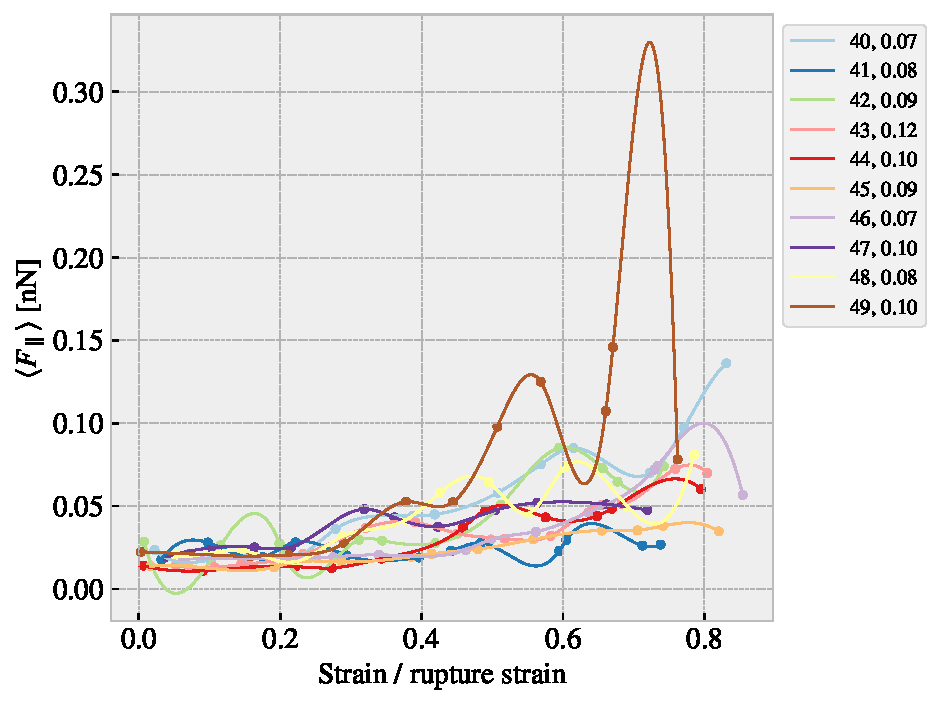
\includegraphics[width=\textwidth]{figures/stretch_profiles/RW/SP_4_RW.pdf}
        \caption{}
        % \label{fig:}
    \end{subfigure}
    \hfill
    \begin{subfigure}[b]{0.49\textwidth}
        \centering
        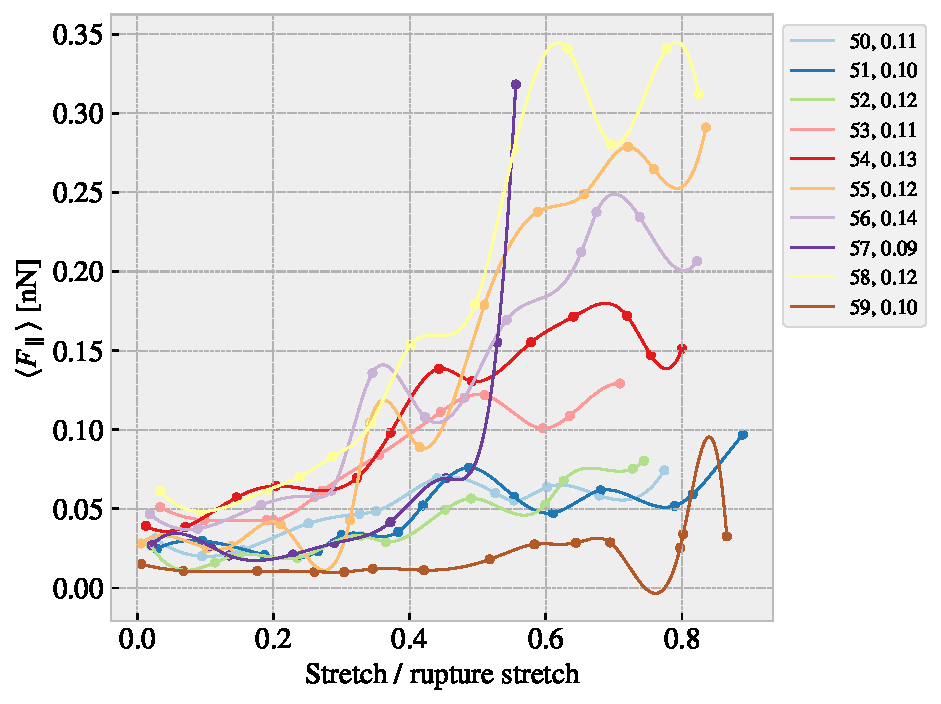
\includegraphics[width=\textwidth]{figures/stretch_profiles/RW/SP_5_RW.pdf}
        \caption{}
        % \label{fig:}
    \end{subfigure}
    \hfill
    \caption{Random walk friction-strain profiles. (The figure continues on the next page)}
\end{figure}


\begin{figure}[H]\ContinuedFloat
    \centering
    \begin{subfigure}[b]{0.49\textwidth}
        \centering
        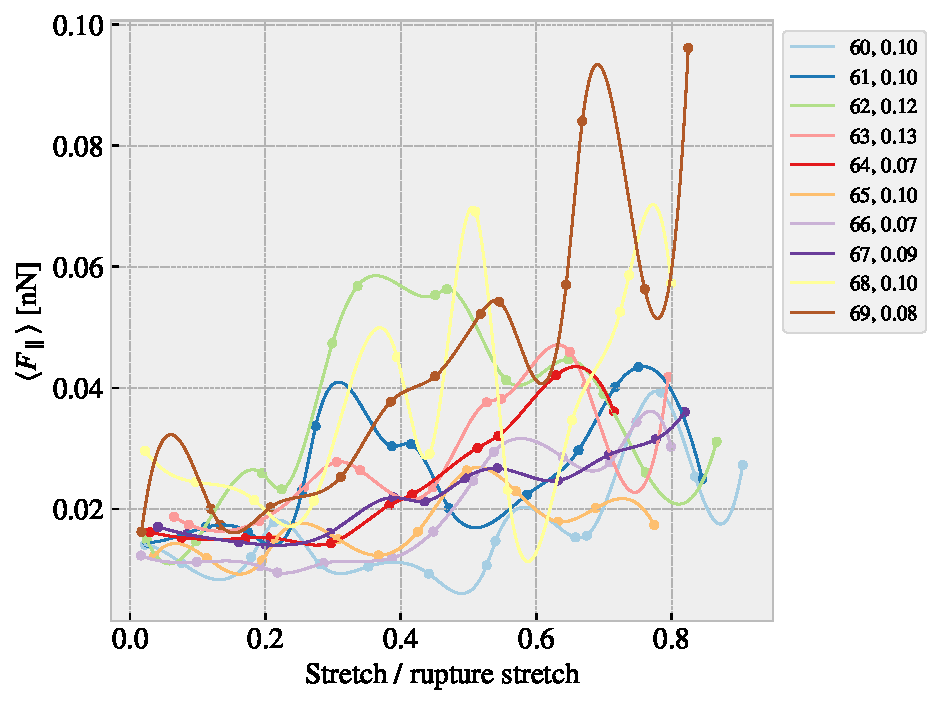
\includegraphics[width=\textwidth]{figures/stretch_profiles/RW/SP_6_RW.pdf}
        \caption{}
        % \label{fig:}
    \end{subfigure}
    \hfill
    \begin{subfigure}[b]{0.49\textwidth}
        \centering
        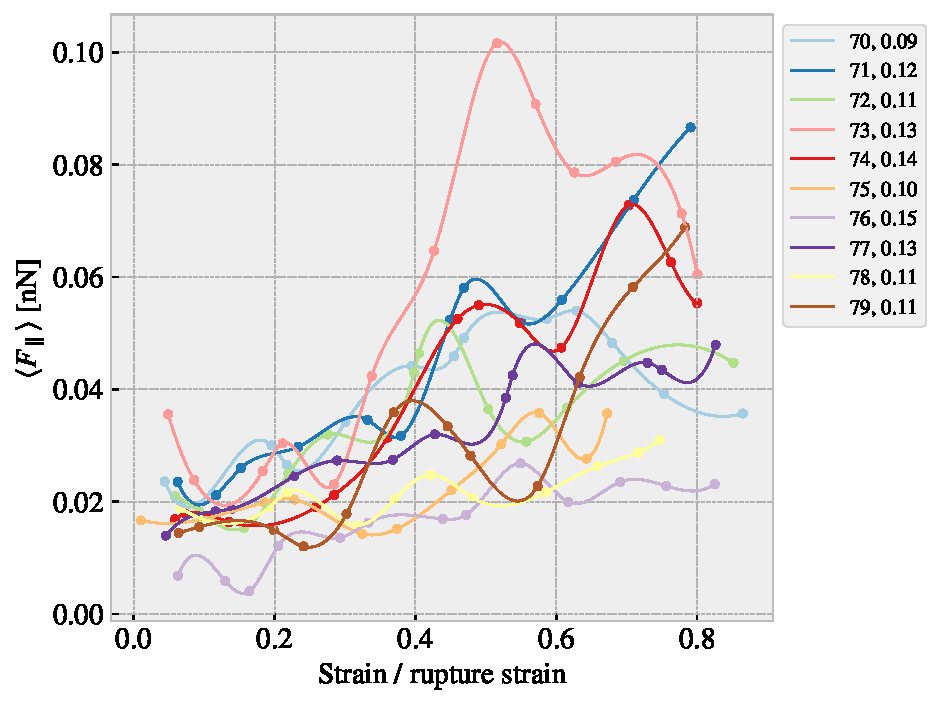
\includegraphics[width=\textwidth]{figures/stretch_profiles/RW/SP_7_RW.pdf}
        \caption{}
        % \label{fig:}
    \end{subfigure}
    \hfill
    \begin{subfigure}[b]{0.49\textwidth}
        \centering
        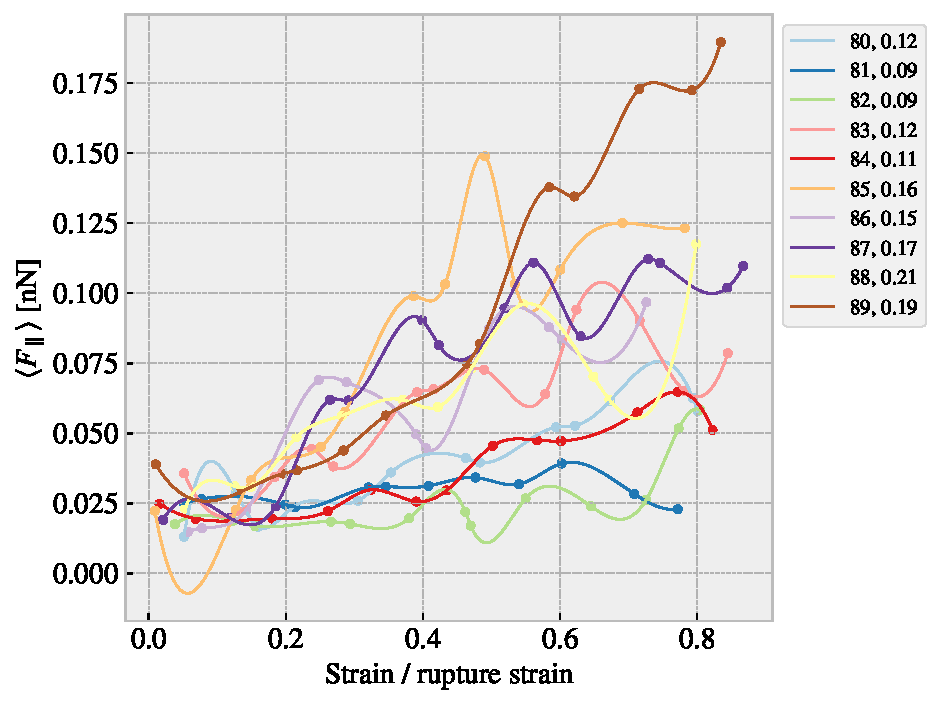
\includegraphics[width=\textwidth]{figures/stretch_profiles/RW/SP_8_RW.pdf}
        \caption{}
        % \label{fig:}
    \end{subfigure}
    \hfill
    \begin{subfigure}[b]{0.49\textwidth}
        \centering
        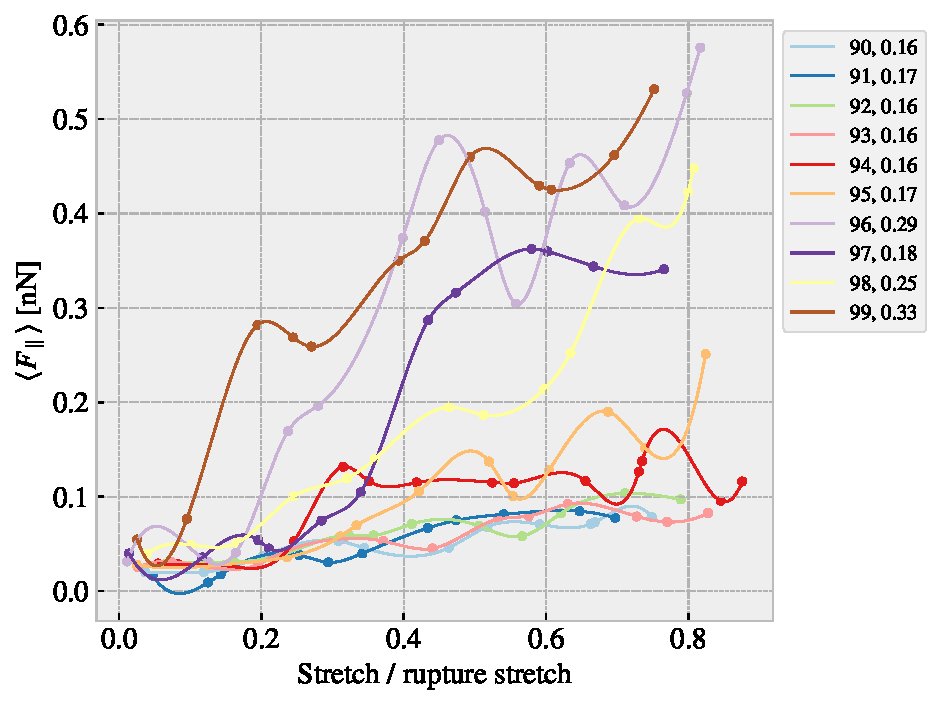
\includegraphics[width=\textwidth]{figures/stretch_profiles/RW/SP_9_RW.pdf}
        \caption{}
        % \label{fig:}
    \end{subfigure}
    \hfill
    \caption{Random walk friction-strain profiles.}\label{fig:fric_strain_RW}
\end{figure}
